\chapter{पृष्ठ, अधिशोषण और विषमांगी उत्प्रेरण}\label{ch:b3:surfaces-catalysis}

कार के नीचे, इस्पात के एक डिब्बे के भीतर, एक सिरेमिक मधुकोश रहता है जिसके हज़ारों
चैनलों पर एक सरंध्र ऑक्साइड का लेप होता है, जिसमें कुछ ग्राम प्लैटिनम,
पैलेडियम और रोडियम होते हैं। एक सेकंड के अंश में, उससे होकर बहने वाली
निकास गैसें अपनी अधिकांश कार्बन मोनोऑक्साइड, अदग्ध हाइड्रोकार्बन और
नाइट्रोजन ऑक्साइड खो देती हैं। गैस में कुछ नहीं होता: इनमें से हर अभिक्रिया
कुछ नैनोमीटर चौड़े धातु कणों के पृष्ठ पर होती है। अधिकांश
रासायनिक उद्योग इसी प्रकार चलता है, उर्वरकों की अमोनिया से लेकर
पेट्रोलियम के भंजन तक। यह अध्याय बताता है कि अणु पृष्ठों से कैसे चिपकते हैं,
वे किसी पृष्ठ का कितना भाग ढकते हैं, पृष्ठीय अभिक्रियाएँ कैसे आगे बढ़ती हैं, और
एक ठोस उत्प्रेरक कैसे बनाया, मापा और देखा जाता है।

\begin{recall}
प्रथम वर्ष के खंड ने उत्प्रेरकों तथा समांगी और विषमांगी उत्प्रेरण के अंतर को
परिभाषित किया, और धातुओं के फलक-केंद्रित घनीय संकुलन का वर्णन किया।
द्वितीय वर्ष के खंड ने किसी उत्प्रेरक के रूपांतरण, वरणात्मकता और
आवर्त आवृत्ति को, तथा ले शातेलिए के सिद्धांत को परिभाषित किया।
\Cref{ch:b3:x-ray-diffraction} ने \omterm{def:b3:x-ray-diffraction:miller}{मिलर सूचकांक} प्रस्तुत किए,
\cref{ch:b3:rate-theories} ने \omterm{thm:b3:rate-theories:eyring}{आयरिंग समीकरण} और
\cref{ch:b3:partition-functions} ने वितरणों की सांख्यिकी।
\end{recall}

\begin{omfigure}
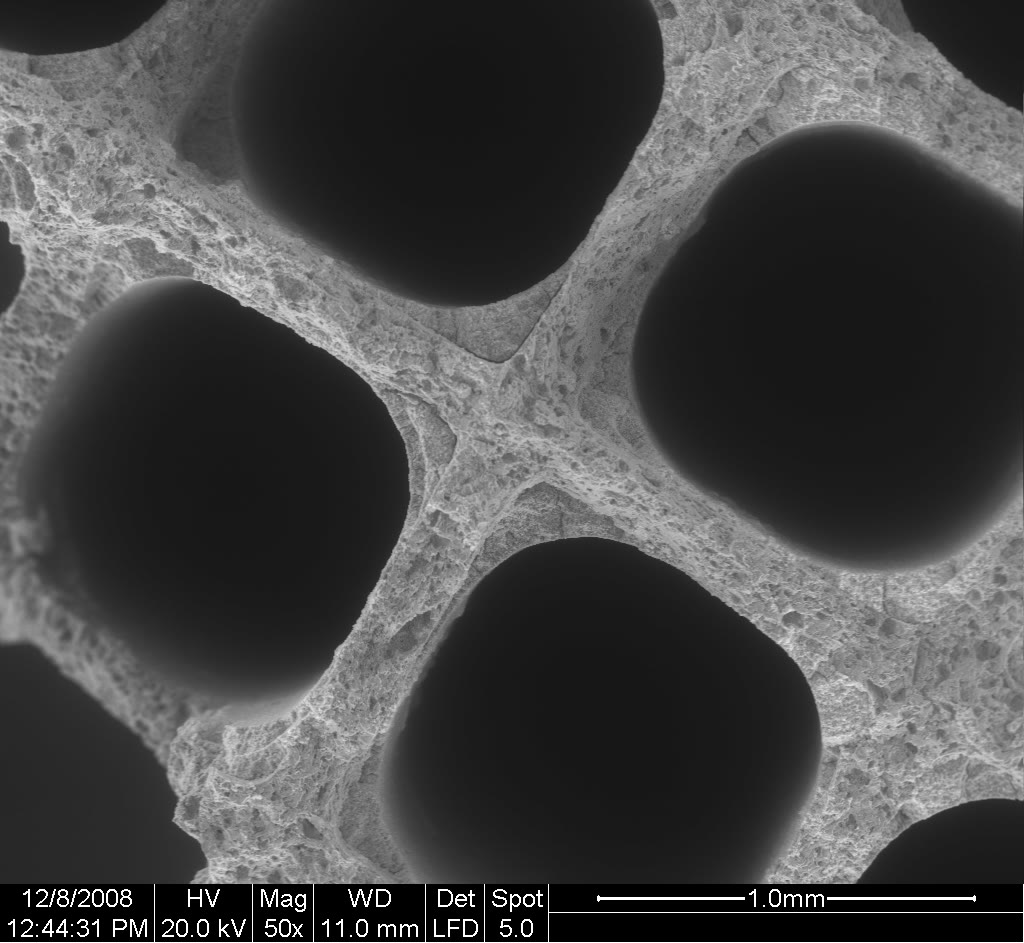
\includegraphics[width=0.48\linewidth]{images/book4/converter-sem.jpg}

{\small क्रमवीक्षी इलेक्ट्रॉन सूक्ष्मदर्शी से देखा गया एक उत्प्रेरकी परिवर्तक का सिरेमिक
मधुकोश (पैमाना-पट्टी \qty{1.0}{mm}): पतली सरंध्र दीवारों से अलग वर्गाकार चैनल,
जो ऑक्साइड लेप और उसके धातु कणों को धारण करती हैं।}
\end{omfigure}

\section{अधिशोषण}

\begin{definition}[अधिशोषण]\label{def:b3:surfaces-catalysis:adsorption}
\emph{अधिशोषण}\index{अधिशोषण} किसी ठोस या द्रव के पृष्ठ पर किसी गैस या
विलेय के अणुओं का संचयन है। अधिशोषित होने वाला अणु
\emph{अधिशोष्य}\index{अधिशोष्य} है, ठोस \emph{अधिशोषक}\index{अधिशोषक};
विपरीत प्रक्रम \emph{विशोषण}\index{विशोषण} है।
\end{definition}

\begin{definition}[भौतिक अधिशोषण, रासायनिक अधिशोषण]\label{def:b3:surfaces-catalysis:physi-chemi}
\emph{भौतिक अधिशोषण}\index{भौतिक अधिशोषण} वान्डरवाल्स बलों द्वारा \omterm{def:b3:surfaces-catalysis:adsorption}{अधिशोषण} है,
जिसकी \omterm{def:b3:surfaces-catalysis:adsorption}{अधिशोषण} एन्थैल्पी अधिक से अधिक कुछ दसियों किलोजूल प्रति मोल होती है,
संघनन एन्थैल्पियों के तुल्य, और अणु में कोई परिवर्तन नहीं होता।
\emph{रासायनिक अधिशोषण}\index{रासायनिक अधिशोषण} पृष्ठ के साथ रासायनिक आबंध बनाता है,
जिसकी एन्थैल्पी लगभग 40 से कई सौ किलोजूल प्रति मोल होती है; यह
अणु को तोड़ सकता है (वियोजी रासायनिक \omterm{def:b3:surfaces-catalysis:adsorption}{अधिशोषण}) और एक परत पर रुक जाता है।
\end{definition}

\begin{omfigure}
\begin{tikzpicture}[font=\small, >=Stealth, x=1cm, y=1cm]
  \draw[->] (0,-2.6) -- (0,1.8) node[anchor=south] {ऊर्जा};
  \draw[->] (0,0) -- (8.0,0) node[anchor=south east] {पृष्ठ से दूरी};
  \draw[omDef, thick] plot[smooth, tension=0.7] coordinates {(1.6,1.6) (2.2,-0.25) (2.8,-0.62) (3.6,-0.35) (5.0,-0.08) (7.5,0)};
  \draw[omThm, thick] plot[smooth, tension=0.6] coordinates {(0.45,1.6) (0.8,-1.2) (1.2,-2.2) (1.7,-1.6) (2.35,-0.15) (2.9,0.9) (3.5,1.5)};
  \node[omDef, anchor=north west, font=\scriptsize] at (3.4,-0.4) {भौतिक अधिशोषित \ce{H2} (पूर्वगामी)};
  \node[omThm, anchor=west, font=\scriptsize] at (1.75,-1.9) {रासायनिक अधिशोषित 2 H};
  \node[omThm, anchor=west, font=\scriptsize, align=left] at (3.55,1.45) {$\mathrm{H} + \mathrm{H}$ की ओर,\\ पृष्ठ से दूर};
  \fill (2.3,-0.2) circle (1.5pt);
  \node[font=\scriptsize] (cr) at (1.25,0.55) {प्रतिच्छेदन};
  \draw[black!60] (cr.south east) -- (2.27,-0.15);
\end{tikzpicture}

{\small धातु पृष्ठ की ओर आते हुए हाइड्रोजन अणु की स्थितिज ऊर्जा
(व्यवस्थात्मक)। अणु पहले उथले \omterm{def:b3:surfaces-catalysis:physi-chemi}{भौतिक अधिशोषण} कूप में गिरता है;
जहाँ यह वक्र अलग-अलग आबंधित दो H परमाणुओं के वक्र को काटता है, वहाँ यह
वियोजित होकर गहरे \omterm{def:b3:surfaces-catalysis:physi-chemi}{रासायनिक अधिशोषण} कूप में जा सकता है। यदि प्रतिच्छेदन शून्य से ऊपर हो,
तो वियोजी \omterm{def:b3:surfaces-catalysis:physi-chemi}{रासायनिक अधिशोषण} सक्रियित होता है।}
\end{omfigure}

धातु कणों के पृष्ठ अधिकतर फलक-केंद्रित घनीय जालक के सबसे सघन फलक, (111) और (100), प्रकट
करते हैं। उन पर कोई \omterm{def:b3:surfaces-catalysis:adsorption}{अधिशोष्य} एक परमाणु के ठीक ऊपर
(शीर्षस्थ), दो के बीच (सेतु) या तीन अथवा चार के बीच के गर्त में बैठ सकता है, और
आबंधन ऊर्जा स्थल-दर-स्थल भिन्न होती है।

\begin{omfigure}
\begin{tikzpicture}[font=\scriptsize]
  % fcc(111): hexagonal layer, spacing 0.6 cm
  \foreach \i in {0,...,5}{\foreach \j in {0,...,4}{
    \shade[ball color=black!25] ({0.6*\i+0.3*\j},{0.52*\j}) circle (0.29);}}
  \fill[omThm] (1.2+0.3*1,0.52) circle (0.07);
  \fill[omDef] ({0.6*2+0.3*2+0.3},{0.52*2}) circle (0.07);
  \fill[black] ({0.6*3+0.3*2+0.3},{0.52*2+0.17}) circle (0.07);
  \fill[black!60!green] ({0.6*1+0.3*3+0.3},{0.52*3-0.17}) circle (0.07);
  \node[anchor=north] at (2.1,-0.45) {(111) फलक};
  % fcc(100): square layer
  \begin{scope}[xshift=5.6cm]
  \foreach \i in {0,...,4}{\foreach \j in {0,...,4}{
    \shade[ball color=black!25] ({0.6*\i},{0.6*\j}) circle (0.29);}}
  \fill[omThm] (1.2,1.2) circle (0.07);
  \fill[omDef] (1.5,1.8) circle (0.07);
  \fill[black] (2.1,0.9) circle (0.07);
  \node[anchor=north] at (1.2,-0.45) {(100) फलक};
  \end{scope}
  \node[anchor=west, align=left] at (9.0,1.6) {\textcolor{omThm}{$\bullet$} शीर्षस्थ\\ \textcolor{omDef}{$\bullet$} सेतु\\
    $\bullet$ गर्त (3- या 4-गुना)\\ \textcolor{black!60!green}{$\bullet$} दूसरा 3-गुना गर्त (111)};
\end{tikzpicture}

{\small एक फलक-केंद्रित घनीय धातु के दो सबसे सघन फलकों के शीर्ष दृश्य,
\omterm{def:b3:surfaces-catalysis:adsorption}{अधिशोषण} स्थलों के साथ: एक परमाणु के ऊपर शीर्षस्थ, दो के बीच सेतु, और गर्तों में:
(111) पर तीन परमाणुओं के बीच (दो प्रकार के, दूसरी परत के किसी परमाणु के ऊपर या नहीं) या
(100) पर चार परमाणुओं के बीच।}
\end{omfigure}

\begin{definition}[भिन्नात्मक आच्छादन, एकलपरत]\label{def:b3:surfaces-catalysis:coverage}
किसी पृष्ठ का \emph{भिन्नात्मक आच्छादन}\index{भिन्नात्मक आच्छादन} $\theta$ उसके
\omterm{def:b3:surfaces-catalysis:adsorption}{अधिशोषण} स्थलों का वह अंश है जो अधिकृत हैं।
\emph{एकलपरत}\index{एकलपरत} \omterm{def:b3:surfaces-catalysis:adsorption}{अधिशोष्य} की एक अकेली पूर्ण परत है, $\theta = 1$।
\end{definition}

\section{समतापी}

\begin{theorem}[लैंगम्यूर समतापी]\label{thm:b3:surfaces-catalysis:langmuir}
यदि किसी पृष्ठ पर सर्वसम, स्वतंत्र स्थल हों, जिनमें से प्रत्येक एक अणु धारण करे, तो
दाब $p$ पर किसी गैस के साथ साम्य पर आच्छादन है
\[
  \theta = \frac{Kp}{1 + Kp},
\]
जहाँ $K$, \omterm{def:b3:surfaces-catalysis:adsorption}{अधिशोषण} साम्य स्थिरांक, केवल
ताप पर निर्भर करता है। यह \emph{लैंगम्यूर समतापी}\index{लैंगम्यूर समतापी} है।
\end{theorem}

\begin{proof}
बलगतिक उपपत्ति। अणु मुक्त स्थलों पर दर $k_ap(1 - \theta)N$ से अधिशोषित होते हैं ($N$
स्थल) और दर $k_d\theta N$ से विशोषित होते हैं। साम्य पर दोनों बराबर होती हैं: $\theta/(1 - \theta)
= (k_a/k_d)p$, जिसे पुनर्व्यवस्थित करने पर $K = k_a/k_d$ के साथ परिणाम मिलता है।

सांख्यिकीय उपपत्ति। $M$ अणुओं को $N$ स्थलों पर $N!/(M!(N - M)!)$ प्रकार से व्यवस्थित किया जा सकता है,
और प्रत्येक अधिशोषित अणु का एक आंतरिक विभाजन फलन $q_{\mathrm s}$ होता है (पृष्ठ के
विरुद्ध उसके कंपन और उसकी आबंधन ऊर्जा)। स्टर्लिंग सूत्र से
अधिशोषित अणुओं का रासायनिक विभव $\mu_{\mathrm s} = -kT\ln\bigl(q_{\mathrm s}\frac{1 - \theta}{\theta}\bigr)$ है;
आदर्श गैस का $\mu_{\mathrm g} = \mu_{\mathrm g}^\circ + kT\ln(p/p^\circ)$ है। साम्य, $\mu_{\mathrm s} = \mu_{\mathrm g}$, देता है
$\theta/(1 - \theta) = q_{\mathrm s}\eu^{\mu_{\mathrm g}^\circ/kT}p/p^\circ$: वही नियम, जिसमें $K$ विभाजन फलनों के
पदों में लिखा गया है।
\end{proof}

निम्न दाब पर $\theta \approx Kp$ (हेनरी क्षेत्र); उच्च दाब पर $\theta \to 1$।
$p = 1/K$ पर आच्छादन आधा होता है।

\begin{proposition}[वियोजी अधिशोषण]\label{prop:b3:surfaces-catalysis:dissociative}
दो स्थलों पर वियोजित होने वाली द्विपरमाणुक गैस के लिए, $\mathrm{H_2} + 2\,{*} \to 2\,\mathrm{H}{*}$ (${*}$: एक मुक्त स्थल),
\[
  \theta = \frac{(Kp)^{1/2}}{1 + (Kp)^{1/2}},
\]
अतः निम्न दाब पर $\theta \propto \sqrt p$।
\end{proposition}

\begin{proof}
\omterm{def:b3:surfaces-catalysis:adsorption}{अधिशोषण} को दो मुक्त स्थल चाहिए, दर $k_ap(1 - \theta)^2$ से; \omterm{def:b3:surfaces-catalysis:adsorption}{विशोषण} के लिए दो
अधिशोषित परमाणुओं का पुनर्संयोजन आवश्यक है, दर $k_d\theta^2$ से। समता से $\theta/(1 - \theta) =
(Kp)^{1/2}$ मिलता है।
\end{proof}

\begin{proposition}[स्पर्धी अधिशोषण]\label{prop:b3:surfaces-catalysis:competitive}
एक ही स्थलों के लिए स्पर्धा करती दो गैसें A और B उन्हें इस प्रकार ढकती हैं
\[
  \theta_{\mathrm A} = \frac{K_{\mathrm A}p_{\mathrm A}}{1 + K_{\mathrm A}p_{\mathrm A} + K_{\mathrm B}p_{\mathrm B}}, \qquad
  \theta_{\mathrm B} = \frac{K_{\mathrm B}p_{\mathrm B}}{1 + K_{\mathrm A}p_{\mathrm A} + K_{\mathrm B}p_{\mathrm B}} .
\]
\end{proposition}

\begin{proof}
प्रत्येक गैस के लिए $k_{a,\mathrm A}p_{\mathrm A}(1 - \theta_{\mathrm A} - \theta_{\mathrm B}) = k_{d,\mathrm A}\theta_{\mathrm A}$, और इसी प्रकार B के लिए। अतः
$\theta_{\mathrm A} = K_{\mathrm A}p_{\mathrm A}\theta_\ast$ और $\theta_{\mathrm B} = K_{\mathrm B}p_{\mathrm B}\theta_\ast$, जहाँ $\theta_\ast = 1 - \theta_{\mathrm A} - \theta_{\mathrm B}$ मुक्त अंश है; जोड़ने पर,
$1 - \theta_\ast = \theta_\ast(K_{\mathrm A}p_{\mathrm A} + K_{\mathrm B}p_{\mathrm B})$।
\end{proof}

\begin{definition}[समआच्छादन अधिशोषण एन्थैल्पी]\label{def:b3:surfaces-catalysis:isosteric}
\emph{समआच्छादन अधिशोषण एन्थैल्पी}\index{समआच्छादन अधिशोषण एन्थैल्पी}
$\Delta_{\mathrm{ads}}H$ नियत आच्छादन पर \omterm{def:b3:surfaces-catalysis:adsorption}{अधिशोषण} की मोलर एन्थैल्पी है,
जो उन दाबों से प्राप्त होती है जो विभिन्न तापों पर वही आच्छादन
देते हैं।
\end{definition}

\begin{proposition}[समआच्छादन एन्थैल्पी]\label{prop:b3:surfaces-catalysis:isosteric}
नियत आच्छादन पर,
\[
  \Bigl(\frac{\partial\ln p}{\partial T}\Bigr)_\theta = -\frac{\Delta_{\mathrm{ads}}H}{RT^2} .
\]
\end{proposition}

\begin{proof}
नियत $\theta$ पर $Kp$ नियत रहता है (लैंगम्यूर पृष्ठ के लिए; व्यापक रूप में वही
तर्क उस आच्छादन पर साम्य स्थिरांक के साथ लागू होता है), अतः $\ln p =
\text{स्थिरांक} - \ln K$। वान्ट हॉफ़ समीकरण से $\dd\ln K/\dd T = \Delta_{\mathrm{ads}}H/RT^2$ (जहाँ $K$
एक मानक दाब के सापेक्ष है)।
\end{proof}

चूँकि \omterm{def:b3:surfaces-catalysis:adsorption}{अधिशोषण} ऊष्माक्षेपी है, उसी आच्छादन के लिए उच्चतर तापों पर उच्चतर दाब
चाहिए: चित्र के समतापी $T$ बढ़ने पर नीचे खिसकते हैं।

\begin{theorem}[BET समतापी]\label{thm:b3:surfaces-catalysis:bet}
यदि अणु क्रमिक परतों में अधिशोषित हों, पहली परत पृष्ठ के अभिलाक्षणिक आबंधन स्थिरांक के साथ
और शेष द्रव के संघनन साम्य के साथ, तो
आपेक्षिक दाब $x = p/p^*$ पर ($p^*$: द्रव \omterm{def:b3:surfaces-catalysis:adsorption}{अधिशोष्य} का वाष्प
दाब) अधिशोषित मात्रा है
\[
  \frac{v}{v_{\mathrm m}} = \frac{cx}{(1 - x)(1 - x + cx)},
\]
जहाँ $v_{\mathrm m}$ एक \omterm{def:b3:surfaces-catalysis:coverage}{एकलपरत} में मात्रा है और $c$ पहली परत में \omterm{def:b3:surfaces-catalysis:adsorption}{अधिशोषण} एन्थैल्पी और
संघनन एन्थैल्पी के अंतर से संबंधित एक स्थिरांक है। यह \emph{BET समतापी}\index{BET समतापी} है (ब्रूनाउअर,
एमेट और टेलर)।
\end{theorem}

\begin{proof}
मान लीजिए $s_i$ पृष्ठ का वह अंश है जो ठीक $i$ परतों से ढका है।
प्रत्येक परत का संतुलन, लैंगम्यूर उपपत्ति की तरह, $s_1 = cxs_0$ और $s_i =
xs_{i-1}$ ($i \ge 2$ के लिए) देता है, अतः $s_i = cx^is_0$। अधिशोषित मात्रा $v/v_{\mathrm m} =
\sum_iis_i/\sum_is_i$ है। $\sum_{i\ge1}x^i = x/(1 - x)$ और $\sum_{i\ge1}ix^i = x/(1 - x)^2$ के साथ:
\[
  \frac{v}{v_{\mathrm m}} = \frac{cs_0\,x/(1 - x)^2}{s_0[1 + cx/(1 - x)]} = \frac{cx}{(1 - x)(1 - x + cx)} .
\]
\end{proof}

पुनर्व्यवस्थित करने पर, $\dfrac{x}{v(1 - x)} = \dfrac{1}{v_{\mathrm m}c} + \dfrac{c - 1}{v_{\mathrm m}c}\,x$: एक सीधी रेखा जिसका ढलान और
अंतःखंड $v_{\mathrm m}$ और $c$ देते हैं, सामान्यतः $0.05 < x < 0.30$ के लिए मान्य।

\begin{definition}[विशिष्ट पृष्ठीय क्षेत्रफल]\label{def:b3:surfaces-catalysis:surface-area}
किसी ठोस का \emph{विशिष्ट पृष्ठीय क्षेत्रफल}\index{विशिष्ट पृष्ठीय क्षेत्रफल} उसके
प्रति इकाई द्रव्यमान पृष्ठीय क्षेत्रफल है, जिसमें उसके रंध्रों की दीवारें भी सम्मिलित हैं।
\end{definition}

\begin{method}[नाइट्रोजन समतापी से विशिष्ट पृष्ठीय क्षेत्रफल]\label{met:b3:surfaces-catalysis:bet-area}
\begin{enumerate}
  \item नमूने को गर्म करते हुए निर्वात में विगैसित कीजिए; उसे द्रव नाइट्रोजन
        (\qty{77}{K}) में ठंडा कीजिए।
  \item 0.05 और 0.30 के बीच के आपेक्षिक दाबों पर अधिशोषित नाइट्रोजन का आयतन
        (मानक परिस्थितियों पर समानीत) मापिए।
  \item $x/(v(1 - x))$ को $x$ के विरुद्ध आलेखित कीजिए; ढलान और अंतःखंड से,
        $v_{\mathrm m} = 1/(\text{ढलान} + \text{अंतःखंड})$ और $c = 1 + \text{ढलान}/\text{अंतःखंड}$।
  \item क्षेत्रफल $= n_{\mathrm m}N_Aa_{\mathrm m}$, जहाँ $n_{\mathrm m}$ \omterm{def:b3:surfaces-catalysis:coverage}{एकलपरत} में मात्रा है और $a_{\mathrm m} = \qty{0.162}{nm^2}$
        एक अधिशोषित नाइट्रोजन अणु का पारंपरिक क्षेत्रफल।
\end{enumerate}
\end{method}

\begin{omfigure}
\begin{tikzpicture}
\begin{axis}[name=la, width=0.31\linewidth, height=5.0cm, xmin=0, xmax=100, ymin=0, ymax=1.05,
  axis lines=left, xlabel={$p$ / kPa}, ylabel={$\theta$}, tick label style={font=\small},
  label style={font=\small}, title={\small लैंगम्यूर}]
\addplot[omDef, thick] table[x=p_kPa, y=T300] {figdata/out/bachelor-3-langmuir-bet-langmuir.dat};
\addplot[omThm, thick] table[x=p_kPa, y=T350] {figdata/out/bachelor-3-langmuir-bet-langmuir.dat};
\node[font=\scriptsize, omDef, anchor=south east] at (axis cs:98,0.92) {\qty{300}{K}};
\node[font=\scriptsize, omThm, anchor=north east] at (axis cs:98,0.45) {\qty{350}{K}};
\end{axis}
\begin{axis}[name=be, at={(la.east)}, anchor=west, xshift=1.9cm, width=0.31\linewidth, height=5.0cm,
  xmin=0, xmax=0.9, ymin=0, ymax=200, axis lines=left, xlabel={$p/p^*$},
  ylabel={$v$ / \unit{cm^3.g^{-1}}}, tick label style={font=\small}, label style={font=\small},
  title={\small BET}]
\addplot[black, thick] table[x=x, y=v] {figdata/out/bachelor-3-langmuir-bet-bet.dat};
\addplot[only marks, mark=*, mark size=1.4pt, omDef] table[x=x, y=v] {figdata/out/bachelor-3-langmuir-bet-data.dat};
\draw[black!40, dashed] (axis cs:0,45) -- (axis cs:0.9,45);
\node[font=\scriptsize, anchor=south east] at (axis cs:0.88,45) {$v_{\mathrm m}$};
\end{axis}
\begin{axis}[at={(be.east)}, anchor=west, xshift=2.1cm, width=0.31\linewidth, height=5.0cm,
  xmin=0, xmax=0.35, ymin=0, ymax=0.0085, axis lines=left, xlabel={$x = p/p^*$},
  ylabel={$x/(v(1 - x))$}, tick label style={font=\small}, label style={font=\small},
  scaled y ticks=false, yticklabel style={/pgf/number format/fixed, /pgf/number format/precision=3},
  title={\small BET आलेख}]
\addplot[black, thin] table[x=x, y=y] {figdata/out/bachelor-3-langmuir-bet-line.dat};
\addplot[only marks, mark=*, mark size=1.4pt, omDef] table[x=x, y=y] {figdata/out/bachelor-3-langmuir-bet-data.dat};
\end{axis}
\end{tikzpicture}

{\small बाएँ: एक मॉडल \omterm{def:b3:surfaces-catalysis:physi-chemi}{रासायनिक अधिशोषण} ($\Delta_{\mathrm{ads}}H = \qty{-40}{kJ/mol}$) के \omterm{thm:b3:surfaces-catalysis:langmuir}{लैंगम्यूर समतापी},
दो तापों पर। मध्य: एक \omterm{thm:b3:surfaces-catalysis:bet}{BET समतापी} (मॉडल, $v_{\mathrm m} = \qty{45}{cm^3.g^{-1}}$, $c = 120$),
सप्ताहांत समस्या के बिंदुओं के साथ; परतें जमती जाती हैं और मात्रा
$p = p^*$ के निकट अपसारी हो जाती है, जहाँ गैस संघनित होती है। दाएँ: उन्हीं बिंदुओं का रैखिक BET आलेख।}
\end{omfigure}

\section{पृष्ठीय अभिक्रियाओं की बलगतिकी}

\begin{definition}[लैंगम्यूर--हिंशेलवुड और एली--राइडील क्रियाविधियाँ]\label{def:b3:surfaces-catalysis:mechanisms}
\emph{लैंगम्यूर--हिंशेलवुड क्रियाविधि}\index{लैंगम्यूर--हिंशेलवुड क्रियाविधि} में
दोनों अभिकारक अधिशोषित होते हैं और पृष्ठ पर अभिक्रिया करते हैं;
\emph{एली--राइडील क्रियाविधि}\index{एली--राइडील क्रियाविधि} में एक अधिशोषित अभिकारक
गैस से आने वाले एक अणु के साथ अभिक्रिया करता है।
\end{definition}

\begin{proposition}[लैंगम्यूर--हिंशेलवुड दर]\label{prop:b3:surfaces-catalysis:lh-rate}
यदि \omterm{def:b3:surfaces-catalysis:adsorption}{अधिशोषण} साम्य तीव्र हों और अधिशोषित A और B की पृष्ठीय अभिक्रिया
दर-निर्धारक हो, तो
\[
  r = k\theta_{\mathrm A}\theta_{\mathrm B} = \frac{kK_{\mathrm A}p_{\mathrm A}K_{\mathrm B}p_{\mathrm B}}{(1 + K_{\mathrm A}p_{\mathrm A} + K_{\mathrm B}p_{\mathrm B})^2},
\]
जो, नियत $p_{\mathrm B}$ पर, तब अधिकतम होती है जब $K_{\mathrm A}p_{\mathrm A} = 1 + K_{\mathrm B}p_{\mathrm B}$, और फिर गिरती है क्योंकि A, B को
पृष्ठ से बाहर धकेल देता है।
\end{proposition}

\begin{proof}
आच्छादन \cref{prop:b3:surfaces-catalysis:competitive} वाले ही हैं। $u =
K_{\mathrm A}p_{\mathrm A}$ और $a = 1 + K_{\mathrm B}p_{\mathrm B}$ रखने पर $r \propto u/(a + u)^2$, जिसका अवकलज $(a - u)/(a + u)^3$
$u = a$ पर शून्य होता है।
\end{proof}

\begin{proposition}[एली--राइडील दर]\label{prop:b3:surfaces-catalysis:er-rate}
यदि अधिशोषित A गैसीय B के साथ अभिक्रिया करे,
\[
  r = k\theta_{\mathrm A}p_{\mathrm B} = \frac{kK_{\mathrm A}p_{\mathrm A}p_{\mathrm B}}{1 + K_{\mathrm A}p_{\mathrm A}},
\]
जो $p_{\mathrm A}$ के साथ एक पठार तक बढ़ती है, बिना किसी अधिकतम के।
\end{proposition}

\begin{proof}
B स्थलों के लिए स्पर्धा नहीं करता: $\theta_{\mathrm A}$ अकेले A का लैंगम्यूर आच्छादन है, और
दर इसके तथा पृष्ठ से B की संघट्ट दर के समानुपाती है, जो
$p_{\mathrm B}$ के समानुपाती है।
\end{proof}

\begin{method}[दाब-निर्भरता से LH या ER]\label{met:b3:surfaces-catalysis:mechanism-from-rate}
\begin{enumerate}
  \item प्रत्येक अभिकारक के दाब के विरुद्ध दर मापिए, दूसरे को नियत
        रखते हुए।
  \item एक अधिकतम, फिर ह्रास (उच्च दाब पर ऋणात्मक कोटि):
        लैंगम्यूर--हिंशेलवुड, अभिकारक स्थलों को घेरकर संदमन करता है।
  \item एक अभिकारक में पठार तक वृद्धि और दूसरे में सभी
        दाबों पर प्रथम कोटि: एली--राइडील।
  \item समस्थानिक अंकन या पृष्ठ स्पेक्ट्रमिकी से पुष्टि कीजिए; अधिकांश उत्प्रेरकी
        अभिक्रियाएँ लैंगम्यूर--हिंशेलवुड प्रकार की निकलती हैं।
\end{enumerate}
\end{method}

\begin{omfigure}
\begin{tikzpicture}
\begin{axis}[width=0.6\linewidth, height=5.4cm, xmin=0, xmax=10, ymin=0, ymax=0.3,
  axis lines=left, xlabel={$p_{\mathrm A}$ (समानीत)}, ylabel={दर (समानीत)},
  tick label style={font=\small}, label style={font=\small},
  legend style={font=\scriptsize, draw=none, at={(1.03,0.98)}, anchor=north west}, legend cell align=left]
\addplot[omDef!50, thick] table[x=pA, y=pB05] {figdata/out/bachelor-3-surface-rates.dat};
\addplot[omDef, thick] table[x=pA, y=pB1] {figdata/out/bachelor-3-surface-rates.dat};
\addplot[black, thick] table[x=pA, y=pB3] {figdata/out/bachelor-3-surface-rates.dat};
\addplot[omThm, thick, dashed] table[x=pA, y=ER] {figdata/out/bachelor-3-surface-rates.dat};
\legend{{LH, $p_{\mathrm B} = 0.5$}, {LH, $p_{\mathrm B} = 1$}, {LH, $p_{\mathrm B} = 3$}, {ER ($\times\frac14$)}}
\end{axis}
\end{tikzpicture}

{\small किसी द्वि-आण्विक पृष्ठीय अभिक्रिया की दरें, A के दाब के विरुद्ध
(समानीत इकाइयाँ, $K_{\mathrm A} = K_{\mathrm B} = 1$)। लैंगम्यूर--हिंशेलवुड: प्रत्येक वक्र $K_{\mathrm A}p_{\mathrm A} =
1 + K_{\mathrm B}p_{\mathrm B}$ पर शिखर बनाता है, फिर A के B को विस्थापित करने पर गिरता है। एली--राइडील (धराशायी, मापित): एक पठार।}
\end{omfigure}

\begin{proposition}[आभासी सक्रियण ऊर्जा]\label{prop:b3:surfaces-catalysis:apparent-ea}
लैंगम्यूर \omterm{def:b3:surfaces-catalysis:adsorption}{अधिशोषण} वाली एकाण्विक पृष्ठीय अभिक्रिया के लिए $r = k\theta = kKp/(1 + Kp)$।
निम्न आच्छादन पर मापी गई सक्रियण ऊर्जा $E_{a,\mathrm{app}} = E_a + \Delta_{\mathrm{ads}}H$ है;
उच्च आच्छादन पर यह $E_a$ है।
\end{proposition}

\begin{proof}
निम्न आच्छादन पर $r \approx kKp$, अतः $\dd\ln r/\dd T = \dd\ln k/\dd T + \dd\ln K/\dd T = (E_a + \Delta_{\mathrm{ads}}H)/RT^2$।
उच्च आच्छादन पर $\theta \approx 1$ और $r \approx k$।
\end{proof}

चूँकि $\Delta_{\mathrm{ads}}H < 0$, विरल रूप से ढके पृष्ठ पर कोई अभिक्रिया अपने
वास्तविक अवरोध से आसान दिखती है: ताप बढ़ाने से पृष्ठीय चरण तेज़ होता है, पर
पृष्ठ खाली हो जाता है।

\begin{definition}[साबातिए सिद्धांत, ज्वालामुखी आलेख]\label{def:b3:surfaces-catalysis:sabatier}
\emph{साबातिए सिद्धांत}\index{साबातिए सिद्धांत} कहता है कि सर्वश्रेष्ठ
उत्प्रेरक अभिकारकों को न बहुत क्षीणता से बाँधता है (वे अधिशोषित या
सक्रियित नहीं होते) और न बहुत दृढ़ता से (उत्पाद नहीं छूटते और स्थलों को अवरुद्ध कर देते हैं)।
उत्प्रेरकों की किसी श्रेणी की सक्रियता का किसी आबंधन ऊर्जा के विरुद्ध
\emph{ज्वालामुखी आलेख}\index{ज्वालामुखी आलेख} मध्यवर्ती आबंधन पर अधिकतम दिखाता है।
\end{definition}

\begin{omfigure}
\begin{tikzpicture}[font=\small, >=Stealth]
  \draw[->] (0,0) -- (7.2,0) node[anchor=north east] {अधिशोष्य की आबंधन प्रबलता};
  \draw[->] (0,0) -- (0,3.6) node[anchor=south] {सक्रियता};
  \draw[omDef, very thick] (0.4,0.3) -- (3.4,3.0) -- (6.6,0.4);
  \node[anchor=south, align=center, font=\scriptsize] at (1.35,2.0) {बहुत क्षीण आबंधन:\\ अभिकारक\\ सक्रियित नहीं};
  \node[anchor=south, align=center, font=\scriptsize] at (5.9,2.0) {बहुत दृढ़ आबंधन:\\ उत्पाद स्थलों को\\ अवरुद्ध करते हैं};
  \node[anchor=south, font=\scriptsize] at (3.4,3.05) {सर्वश्रेष्ठ उत्प्रेरक};
\end{tikzpicture}

{\small एक \omterm{def:b3:surfaces-catalysis:sabatier}{ज्वालामुखी आलेख} (गुणात्मक): उत्प्रेरकों की एक श्रेणी की सक्रियता,
उस प्रबलता के विरुद्ध जिससे वे किसी मुख्य मध्यवर्ती को बाँधते हैं।}
\end{omfigure}

\section{औद्योगिक उत्प्रेरक}

\begin{definition}[उत्प्रेरक अभिकल्पन]\label{def:b3:surfaces-catalysis:catalyst-design}
\emph{उत्प्रेरक आधार}\index{उत्प्रेरक आधार} एक सरंध्र, उच्च-क्षेत्रफल ठोस है
(ऐलुमिना, सिलिका, कार्बन) जो सक्रिय प्रावस्था के छोटे कणों को धारण करता है।
\emph{वर्धक}\index{वर्धक} एक योज्य है, अकेले निष्क्रिय, जो
सक्रियता, वरणात्मकता या स्थायित्व बढ़ाता है। \emph{उत्प्रेरक विष}\index{उत्प्रेरक विष}
वह पदार्थ है जो \omterm{def:b3:complex-kinetics:enzyme}{सक्रिय स्थलों} से दृढ़ता से बँधकर उन्हें अवरुद्ध कर देता है।
\emph{धातु परिक्षेपण}\index{धातु परिक्षेपण} $D$ धातु के उन परमाणुओं का अंश है
जो पृष्ठ पर स्थित हैं। \emph{सिंटरन}\index{सिंटरन} उच्च ताप पर
कणों की वृद्धि है, जो परिक्षेपण को घटाती है।
\end{definition}

\begin{method}[हाइड्रोजन रासायनिक अधिशोषण से परिक्षेपण और कण आकार]\label{met:b3:surfaces-catalysis:dispersion}
\begin{enumerate}
  \item उत्प्रेरक को हाइड्रोजन में अपचयित कीजिए, निर्वातित कीजिए, और धातु पर रासायनिक अधिशोषित
        \ce{H2} का आयतन (मानक परिस्थितियों पर समानीत) मापिए; आधार
        कुछ भी अधिशोषित नहीं करता।
  \item प्रति पृष्ठीय धातु परमाणु एक H परमाणु मानिए: $D = n_{\ce{H}}/n_{\text{धातु}}$।
  \item व्यास $d$ के गोलों के लिए $D = 6(v_{\mathrm{at}}/a_{\mathrm{at}})/d$, जहाँ $v_{\mathrm{at}}$ स्थूल में प्रति परमाणु
        आयतन है और $a_{\mathrm{at}}$ प्रति पृष्ठीय परमाणु क्षेत्रफल; अतः $d = 6v_{\mathrm{at}}/(a_{\mathrm{at}}D)$।
\end{enumerate}
\end{method}

अमोनिया संश्लेषण, $\ce{N2 + 3 H2 <=> 2 NH3}$, लगभग 400 से \qty{500}{\celsius} और 100 से
\qty{300}{bar} पर पोटैशियम ऑक्साइड और ऐलुमिना से वर्धित आयरन पर चलता है: ऐलुमिना
आयरन क्रिस्टलकों को \omterm{def:b3:surfaces-catalysis:catalyst-design}{सिंटरन} से बचाता है, पोटैशियम सक्रियता बढ़ाता है।
दर-निर्धारक चरण \ce{N2} का वियोजी \omterm{def:b3:surfaces-catalysis:physi-chemi}{रासायनिक अधिशोषण} है, जिसका त्रिक
आबंध तोड़ना सबसे कठिन है। प्रति वर्ष लगभग 15 करोड़ टन नाइट्रोजन इस प्रकार
स्थिर की जाती है।
% ledger: nh3:world-2024
वैनेडियम(V) ऑक्साइड पर, जो पोटैशियम सल्फ़ेट से वर्धित होता है, \ce{SO2} का \ce{SO3} में
ऑक्सीकरण सल्फ़्यूरिक अम्ल निर्माण का मुख्य चरण है।

पेट्रोल इंजनों का त्रिमार्गी परिवर्तक CO और हाइड्रोकार्बनों का ऑक्सीकरण तथा
नाइट्रोजन ऑक्साइडों का अपचयन एक साथ करता है, प्लैटिनम और पैलेडियम (ऑक्सीकरण)
तथा रोडियम (NO का अपचयन) पर, जो सीरियम ऑक्साइड सहित ऐलुमिना पर परिक्षेपित होते हैं; सीरियम ऑक्साइड
ऑक्सीजन का भंडारण और मोचन करता है। यह केवल रससमीकरणमितीय वायु--ईंधन अनुपात के आसपास की
एक संकीर्ण खिड़की में ही कार्य करता है: अधिक वायु होने पर NO अपचयित नहीं होता,
अधिक ईंधन होने पर CO ऑक्सीकृत नहीं होता; निकास में एक ऑक्सीजन संवेदक
इंजन को खिड़की में बनाए रखता है। सीसायुक्त ईंधन का सीसा धातु को विषाक्त कर देता है, जो
सीसायुक्त पेट्रोल के लुप्त होने का एक कारण है। ज़िओलाइट, अर्थात् आण्विक आकार के रंध्रों
और अम्लीय स्थलों वाले क्रिस्टलीय ऐलुमिनोसिलिकेट, भारी
तेल प्रभाजों के बड़े अणुओं का पेट्रोल में भंजन करते हैं और केवल उन्हीं अणुओं को प्रवेश देते हैं जो उनके चैनलों में समा सकें।

\begin{omfigure}
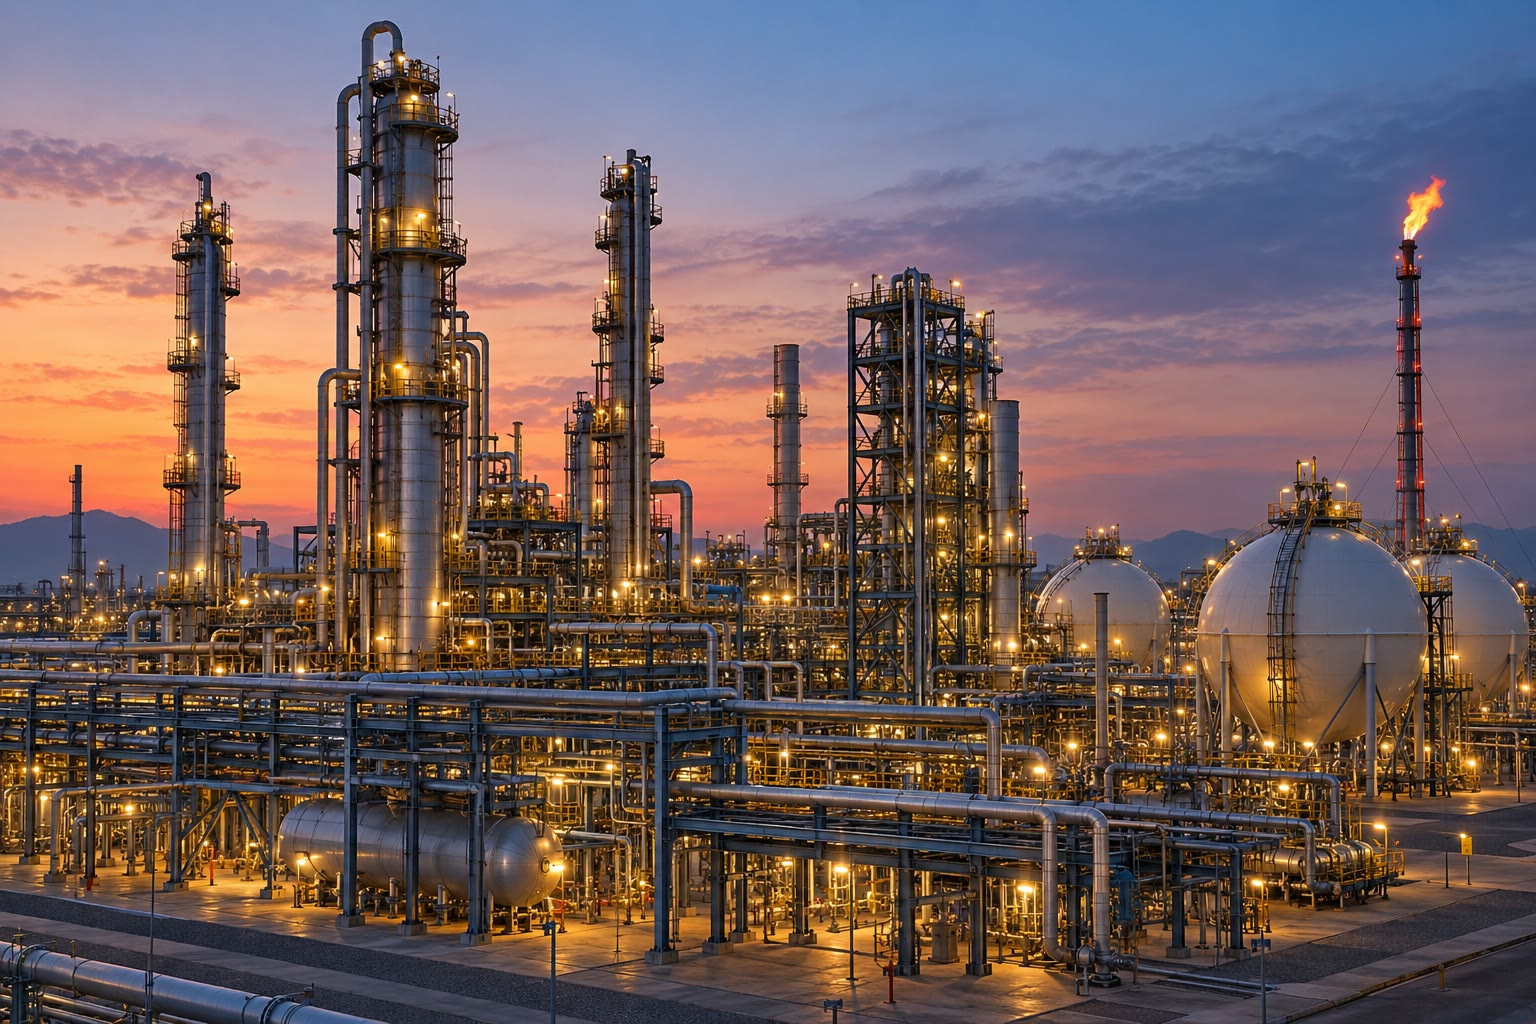
\includegraphics[width=0.6\linewidth]{images/book4/ai/b3-16-ammonia-plant.jpg}

{\small एक अमोनिया संश्लेषण संयंत्र। इसके केंद्र में स्थित रिएक्टर में टनों
वर्धित आयरन उत्प्रेरक होता है; संयंत्र का अधिकांश भाग हाइड्रोजन तैयार करता है और
अरूपांतरित गैस का पुनर्चक्रण करता है।}
\end{omfigure}

\section{पृष्ठों का अवलोकन}

\begin{definition}[तापीय विशोषण स्पेक्ट्रमिकी]\label{def:b3:surfaces-catalysis:tpd}
\emph{तापीय विशोषण स्पेक्ट्रमिकी}\index{तापीय विशोषण स्पेक्ट्रमिकी}
\omterm{def:b3:surfaces-catalysis:adsorption}{अधिशोष्य} वाले पृष्ठ को नियत दर से गर्म करती है और विशोषित होने वाली गैस को
द्रव्यमान स्पेक्ट्रममापी से अभिलिखित करती है; प्रत्येक आबंधन अवस्था एक शिखर देती है, जिसका
ताप उसकी \omterm{def:b3:surfaces-catalysis:adsorption}{विशोषण} सक्रियण ऊर्जा के साथ बढ़ता है।
\end{definition}

\omterm{def:b3:surfaces-catalysis:adsorption}{विशोषण} शिखर की स्थिति \omterm{def:b3:surfaces-catalysis:adsorption}{विशोषण} ऊर्जा देती है (प्रथम-कोटि
\omterm{def:b3:surfaces-catalysis:adsorption}{विशोषण} के लिए $E_d \approx RT_{\mathrm p}[\ln(\nu T_{\mathrm p}/\beta) - 3.64]$, जहाँ $\beta$ तापन दर है और $\nu \approx \qty{e13}{s^{-1}}$,
स्वीकृत), उसका क्षेत्रफल अधिशोषित मात्रा। X-किरणों से
प्रकाशइलेक्ट्रॉन स्पेक्ट्रमिकी (XPS) पृष्ठीय परमाणुओं के क्रोड इलेक्ट्रॉनों की आबंधन ऊर्जाएँ मापती है,
जो प्रथम कुछ नैनोमीटरों में तत्वों और उनकी ऑक्सीकरण अवस्थाओं की पहचान
कराती हैं। क्रमवीक्षी \omterm{def:b3:quantum-model-systems:tunnelling}{सुरंगन} सूक्ष्मदर्शी एक नुकीली नोक को किसी चालक पृष्ठ से
नैनोमीटर के कुछ दशांश ऊपर घुमाता है; \omterm{def:b3:quantum-model-systems:tunnelling}{सुरंगन} धारा
(\cref{ch:b3:quantum-model-systems}) प्रत्येक अतिरिक्त \qty{0.1}{nm} दूरी पर लगभग परिमाण की
एक कोटि गिर जाती है, अतः क्रमवीक्षण करते हुए इसे नियत रखने से
पृष्ठ का परमाणु-दर-परमाणु मानचित्र बनता है।

\begin{inthelab}[एक BET मापन]
लगभग \qty{0.2}{g} नमूना एक बल्ब वाली काँच की नली में तौला जाता है, घंटों तक
निर्वात में 150 से \qty{300}{\celsius} पर विगैसित किया जाता है, फिर तौला जाता है, और
उपकरण पर चढ़ाया जाता है, बल्ब द्रव नाइट्रोजन के ड्यूअर में डूबा रहता है। उपकरण
नाइट्रोजन को छोटी खुराकों में प्रविष्ट करता है और प्रत्येक के बाद साम्य दाब मापता है,
गैस संतुलन से अधिशोषित मात्रा निकालता है; नली का मृत आयतन
हीलियम से मापा जाता है, जो अधिशोषित नहीं होती।
\end{inthelab}

\begin{safety}{\ghs[0.7cm]{GHS06}\ghs[0.7cm]{GHS07}\ghs[0.7cm]{GHS08}\ghs[0.7cm]{GHS09}}
% ledger: ghs4:V2O5, ghs4:Ni
अपचयित धातु उत्प्रेरक (किसी आधार पर सूक्ष्म विभाजित निकेल, पैलेडियम या प्लैटिनम,
हाइड्रोजन में ताज़ा अपचयित) वायु के संपर्क में प्रज्वलित हो सकते हैं: उन्हें
अक्रिय गैस के अधीन सँभाला जाता है और भंडारण से पहले निष्क्रियित किया जाता है। निकेल त्वचा
सुग्राहीकारक और संदिग्ध कैंसरजन है; वैनेडियम(V) ऑक्साइड साँस द्वारा लेने
और निगलने पर विषैला है और कैंसर उत्पन्न कर सकता है। उत्प्रेरक चूर्ण एक
संवातित आवरण में तौले जाते हैं।
\end{safety}

\begin{history}[लैंगम्यूर और अमोनिया उत्प्रेरक]
इरविंग लैंगम्यूर ने, एक औद्योगिक प्रयोगशाला में बल्बों पर कार्य करते हुए,
1916--1918 में अपना समतापी इस विचार से व्युत्पन्न किया कि अधिशोषित गैसें एक
अणु मोटी परत बनाती हैं, और अपने पृष्ठ रसायन के लिए उन्हें रसायन का 1932 का
नोबेल पुरस्कार मिला। कुछ वर्ष पहले, आल्विन मिटाश ने
एक व्यावहारिक अमोनिया उत्प्रेरक की खोज संगठित की थी: वर्धित आयरन उत्प्रेरक, जो
आज भी प्रयोग में है, चुने जाने से पहले हज़ारों संघटनों का छोटे
उच्च-दाब रिएक्टरों में परीक्षण किया गया। यह उत्प्रेरकों की पहली क्रमबद्ध छानबीनों में से एक थी।
\end{history}

\section{अभ्यास}

\begin{exercise}[$\star$]\label{exo:b3:surfaces-catalysis:1}
एक गैस \qty{2.0}{kPa} पर किसी लैंगम्यूर पृष्ठ का 40\,\% ढकती है। $K$ और
\qty{10}{kPa} पर आच्छादन परिकलित कीजिए।
\end{exercise}

\begin{exercise}[$\star$]\label{exo:b3:surfaces-catalysis:2}
किसी धातु पर दो \omterm{def:b3:surfaces-catalysis:adsorption}{अधिशोषण} एन्थैल्पियाँ मापी जाती हैं: $-20$ और \qty{-150}{kJ/mol}। कौन
\omterm{def:b3:surfaces-catalysis:physi-chemi}{भौतिक अधिशोषण} है, कौन \omterm{def:b3:surfaces-catalysis:physi-chemi}{रासायनिक अधिशोषण}? कौन वियोजी हो सकता है?
\end{exercise}

\begin{exercise}[$\star$]\label{exo:b3:surfaces-catalysis:3}
किसी फलक-केंद्रित घनीय धातु के एक (100) फलक और एक (111) फलक के प्रति पृष्ठीय परमाणु
शीर्षस्थ, सेतु और गर्त स्थल गिनिए।
\end{exercise}

\begin{exercise}[$\star$]\label{exo:b3:surfaces-catalysis:4}
एक उत्प्रेरक प्रति ग्राम प्रति सेकंड \qty{3.0e-6}{mol} अभिकारक रूपांतरित करता है और उस पर
प्रति ग्राम \qty{1.5e-5}{mol} पृष्ठीय स्थल हैं। आवर्त आवृत्ति परिकलित कीजिए।
\end{exercise}

\begin{exercise}[$\star\star$]\label{exo:b3:surfaces-catalysis:5}
हाइड्रोजन \qty{1.0}{kPa} पर $\theta = 0.10$ के साथ वियोजी रूप से अधिशोषित होती है। \qty{4.0}{kPa} पर $\theta$ परिकलित कीजिए।
\end{exercise}

\begin{exercise}[$\star\star$]\label{exo:b3:surfaces-catalysis:6}
CO ($K = \qty{10}{kPa^{-1}}$) और \ce{O2} ($K = \qty{0.5}{kPa^{-1}}$, इस सरल मॉडल में अवियोजी)
1.0 और \qty{5.0}{kPa} पर किसी प्लैटिनम पृष्ठ के स्थलों के लिए स्पर्धा करते हैं। दोनों
आच्छादन परिकलित कीजिए और CO ऑक्सीकरण की दर पर टिप्पणी कीजिए।
\end{exercise}

\begin{exercise}[$\star\star$]\label{exo:b3:surfaces-catalysis:7}
\qty{300}{K} पर \qty{1.0}{kPa} पर प्राप्त होने वाले आच्छादन के लिए \qty{350}{K} पर \qty{8.0}{kPa} चाहिए। \omterm{def:b3:surfaces-catalysis:isosteric}{समआच्छादन
अधिशोषण एन्थैल्पी} परिकलित कीजिए।
\end{exercise}

\begin{exercise}[$\star\star$]\label{exo:b3:surfaces-catalysis:8}
% ledger: sa:N2.am, const:Vm1, const:NA
एक सक्रियित कार्बन के लिए $v_{\mathrm m} = \qty{120}{cm^3.g^{-1}}$ है (मानक परिस्थितियाँ, 273.15 K और
\qty{101.325}{kPa})। इसका BET क्षेत्रफल परिकलित कीजिए।
\end{exercise}

\begin{exercise}[$\star\star$]\label{exo:b3:surfaces-catalysis:9}
प्लैटिनम पर $\ce{2 CO + O2 -> 2 CO2}$ की दर, $p(\ce{CO})$ बढ़ने पर, $p(\ce{O2})$ नियत रखते हुए,
बढ़ती है, एक अधिकतम से गुज़रती है और गिरती है। यह किस क्रियाविधि का संकेत देता है, और CO
अभिक्रिया का संदमन क्यों करता है?
\end{exercise}

\begin{exercise}[$\star\star\star$]\label{exo:b3:surfaces-catalysis:10}
एक पृष्ठीय अभिक्रिया की वास्तविक सक्रियण ऊर्जा \qty{100}{kJ/mol} है; अभिकारक के लिए
$\Delta_{\mathrm{ads}}H = \qty{-60}{kJ/mol}$। निम्न और उच्च आच्छादन पर कौन-सी सक्रियण ऊर्जा मापी जाती है?
विस्तृत परास में $\ln r$ का $1/T$ के विरुद्ध रेखाचित्र बनाइए।
\end{exercise}

\begin{exercise}[$\star\star\star$]\label{exo:b3:surfaces-catalysis:11}
सल्फ़र एक निकेल उत्प्रेरक पर 0.10 (प्रति पृष्ठीय Ni सल्फ़र परमाणु) के आच्छादन के साथ
अधिशोषित होता है, और प्रत्येक सल्फ़र परमाणु चार स्थलों को अवरुद्ध करता है। एक मुक्त स्थल चाहने वाली
अभिक्रिया के लिए सक्रियता का कितना अंश शेष रहता है? दो संलग्न मुक्त स्थल चाहने वाली के लिए (अवरुद्ध
स्थलों को यादृच्छिक रूप से स्थित मानिए)?
\end{exercise}

\begin{exercise}[$\star\star\star$]\label{exo:b3:surfaces-catalysis:12}
अमोनिया संश्लेषण के लिए तीन धातुएँ परमाणुक नाइट्रोजन को
$-150$, $-250$ और \qty{-400}{kJ/mol} की एन्थैल्पियों से बाँधती हैं (अभ्यास के आँकड़े)। \omterm{def:b3:surfaces-catalysis:sabatier}{साबातिए
सिद्धांत} के आधार पर, कौन संभवतः सर्वश्रेष्ठ उत्प्रेरक है, और अन्य दो को क्या सीमित करता है?
\end{exercise}

\section{समस्या: एक उत्प्रेरक का मापन}

\begin{problem}[{सप्ताहांत समस्या --- एक उत्प्रेरक का मापन: एक आधारित
प्लैटिनम उत्प्रेरक का BET क्षेत्रफल, हाइड्रोजन रासायनिक अधिशोषण से उसका धातु परिक्षेपण और कण आकार,
और एक हाइड्रोजनीकरण की आवर्त आवृत्ति}]
\label{pb:b3:surfaces-catalysis:1}
% ledger: sa:N2.am, lat:Pt, aw:Pt, const:Vm1, const:NA
एक उत्प्रेरक में ऐलुमिना पर द्रव्यमान से 1.00\,\% प्लैटिनम है। समस्या के आँकड़े:
\qty{77}{K} पर नाइट्रोजन समतापी (मानक परिस्थितियों, 273.15 K और
\qty{101.325}{kPa}, पर आयतन, प्रति ग्राम):
\begin{center}\small
\begin{tabular}{lcccccc}
\hline
$x = p/p^*$ & 0.05 & 0.10 & 0.15 & 0.20 & 0.25 & 0.30 \\
$v$ / \unit{cm^3.g^{-1}} & 41.2 & 46.1 & 51.1 & 54.1 & 58.9 & 62.9 \\ \hline
\end{tabular}
\end{center}
प्लैटिनम पर रासायनिक अधिशोषित \ce{H2}: प्रति ग्राम उत्प्रेरक \qty{0.205}{cm^3}। एक हाइड्रोजनीकरण
प्रति ग्राम उत्प्रेरक प्रति सेकंड \qty{2.0e-5}{mol} पर चलता है। प्लैटिनम: $M = \qty{195.08}{g/mol}$, फलक-केंद्रित घनीय,
$a = \qty{392.3}{pm}$; मानक परिस्थितियों पर किसी गैस का मोलर आयतन \qty{22414}{cm^3/mol};
$a_{\mathrm m}(\ce{N2}) = \qty{0.162}{nm^2}$।

\medskip\noindent\textbf{भाग I --- BET आलेख।}
\begin{enumerate}
  \item समतापी \qty{77}{K} पर क्यों मापा जाता है?
  \item केवल 0.05 और 0.30 के बीच के आपेक्षिक दाब ही क्यों प्रयुक्त होते हैं?
  \item प्रत्येक बिंदु के लिए $x/(v(1 - x))$ परिकलित कीजिए।
  \item न्यूनतम-वर्ग रेखा का ढलान \num{0.02205} और अंतःखंड \num{0.000180} है
        (\unit{g.cm^{-3}} में)। $v_{\mathrm m}$ निकालिए।
  \item $c$ निकालिए। बड़े $c$ का क्या अर्थ है?
  \item अंतःखंड इतनी खराब तरह से क्यों निर्धारित होता है, और क्या $v_{\mathrm m}$ के लिए इसका महत्त्व है?
\end{enumerate}

\medskip\noindent\textbf{भाग II --- क्षेत्रफल।}
\begin{enumerate}[resume]
  \item प्रति ग्राम \omterm{def:b3:surfaces-catalysis:coverage}{एकलपरत} में नाइट्रोजन की मात्रा परिकलित कीजिए।
  \item \omterm{def:b3:surfaces-catalysis:surface-area}{विशिष्ट पृष्ठीय क्षेत्रफल} परिकलित कीजिए।
  \item ठोस का कौन-सा भाग इस क्षेत्रफल का लगभग सारा अंश प्रदान करता है?
  \item ज़िओलाइट जैसे सूक्ष्मरंध्री ठोसों के लिए BET विधि विफल क्यों होती है?
\end{enumerate}

\medskip\noindent\textbf{भाग III --- परिक्षेपण और कण आकार।}
\begin{enumerate}[resume]
  \item प्रति ग्राम रासायनिक अधिशोषित H परमाणुओं की मात्रा परिकलित कीजिए।
  \item प्रति ग्राम प्लैटिनम की मात्रा परिकलित कीजिए।
  \item परिक्षेपण निकालिए।
  \item स्थूल में प्रति Pt परमाणु आयतन परिकलित कीजिए।
  \item (111), (100) और (110) फलकों पर औसत प्रति पृष्ठीय परमाणु क्षेत्रफल
        \qty{0.0807}{nm^2} है। (111) का मान, $\frac{\sqrt3}{4}a^2$, जाँचिए।
  \item दिखाइए कि गोलों के लिए $d = 6v_{\mathrm{at}}/(a_{\mathrm{at}}D)$।
  \item माध्य कण व्यास परिकलित कीजिए।
  \item कौन-सी मान्यताएँ इस परिणाम को सीमित करती हैं?
\end{enumerate}

\medskip\noindent\textbf{भाग IV --- सक्रियता।}
\begin{enumerate}[resume]
  \item प्रति पृष्ठीय Pt परमाणु आवर्त आवृत्ति परिकलित कीजिए।
  \item प्रति ग्राम प्लैटिनम दर परिकलित कीजिए।
  \item यदि नियत आवर्त आवृत्ति पर कण सिंटरित होकर \qty{10}{nm} के हो जाएँ, तो प्रति ग्राम दर
        किस गुणक से गिरेगी?
  \item कण आकार के साथ बदलने वाली आवर्त आवृत्ति क्या प्रकट करेगी?
  \item उत्प्रेरकों की तुलना प्रति ग्राम दर के बजाय आवर्त आवृत्ति से क्यों की जाती
        है?
  \item परिणाम बताइए: प्लैटिनम कणों का माध्य व्यास।
\end{enumerate}
\end{problem}
